\documentclass[10pt,onecolumn]{article}
\usepackage[letterpaper,margin=0.75in]{geometry}
\usepackage{graphicx}
\usepackage{microtype}
\renewcommand{\thefigure}{S\arabic{figure}}

\title{Supplementary Figures\\\large Verifying LLM-extracted text with token alignment}
\author{A. Sina Booeshaghi and Aaron Streets}
\date{}

\begin{document}
\maketitle

\begin{figure}[h!]
    \centering
    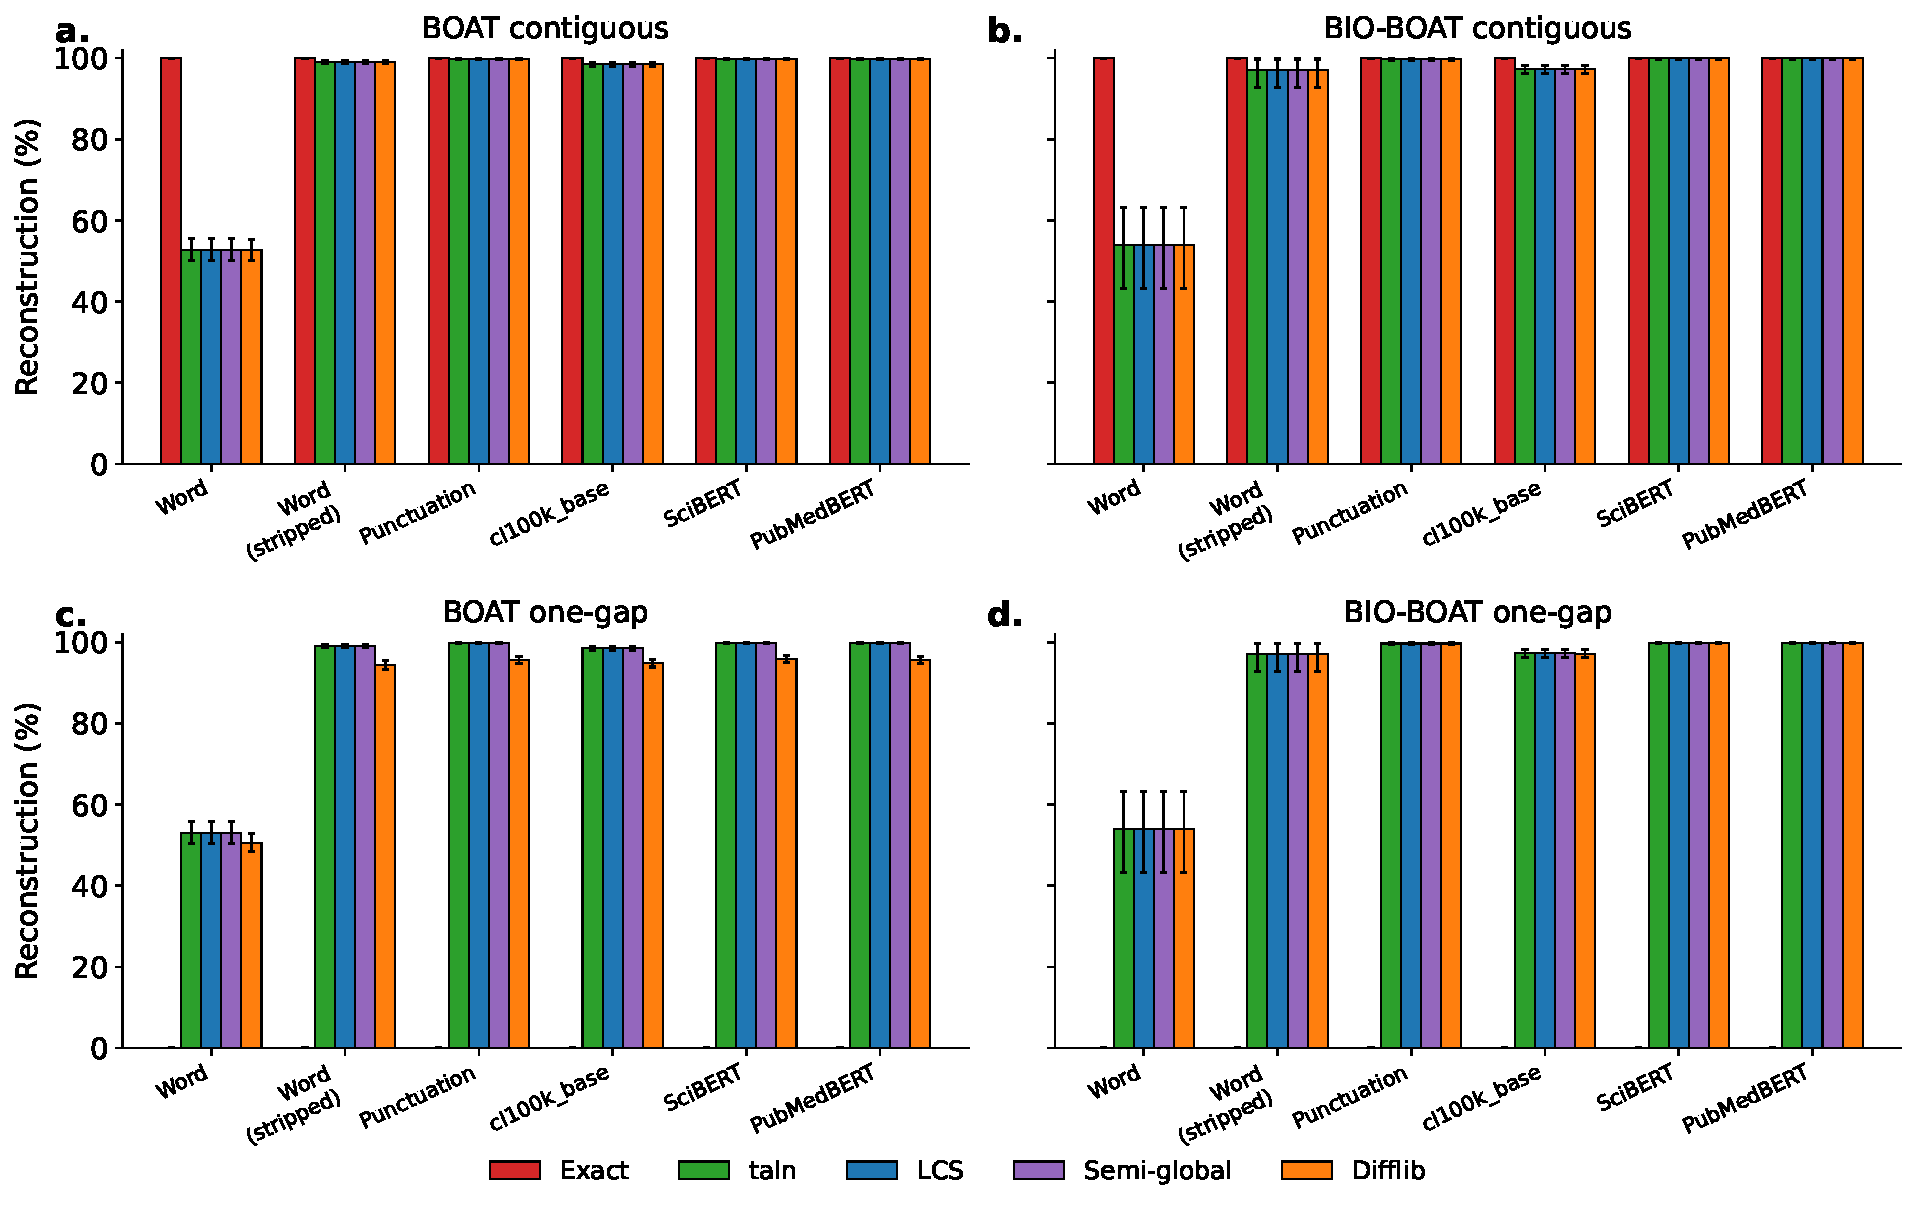
\includegraphics[width=\linewidth]{../../shared/figures/reconstruction_accuracy.pdf}
    \caption{\textbf{Reconstruction accuracy across methods and tokenizers.} Held-out reconstruction for exact string matching, \texttt{taln}, LCS, semi-global alignment, and \texttt{difflib} under six tokenizers, with document-clustered 95\% confidence intervals. \textbf{a.} \texttt{BOAT} contiguous (n=4,313). \textbf{b.} \texttt{BIO-BOAT} contiguous (n=1,259). \textbf{c.} \texttt{BOAT} one-gap (n=4,284). \textbf{d.} \texttt{BIO-BOAT} one-gap (n=1,259). Exact string matching does not depend on the tokenizer and is shown at every position.}
    \label{fig:s1}
\end{figure}

\begin{figure}[h!]
    \centering
    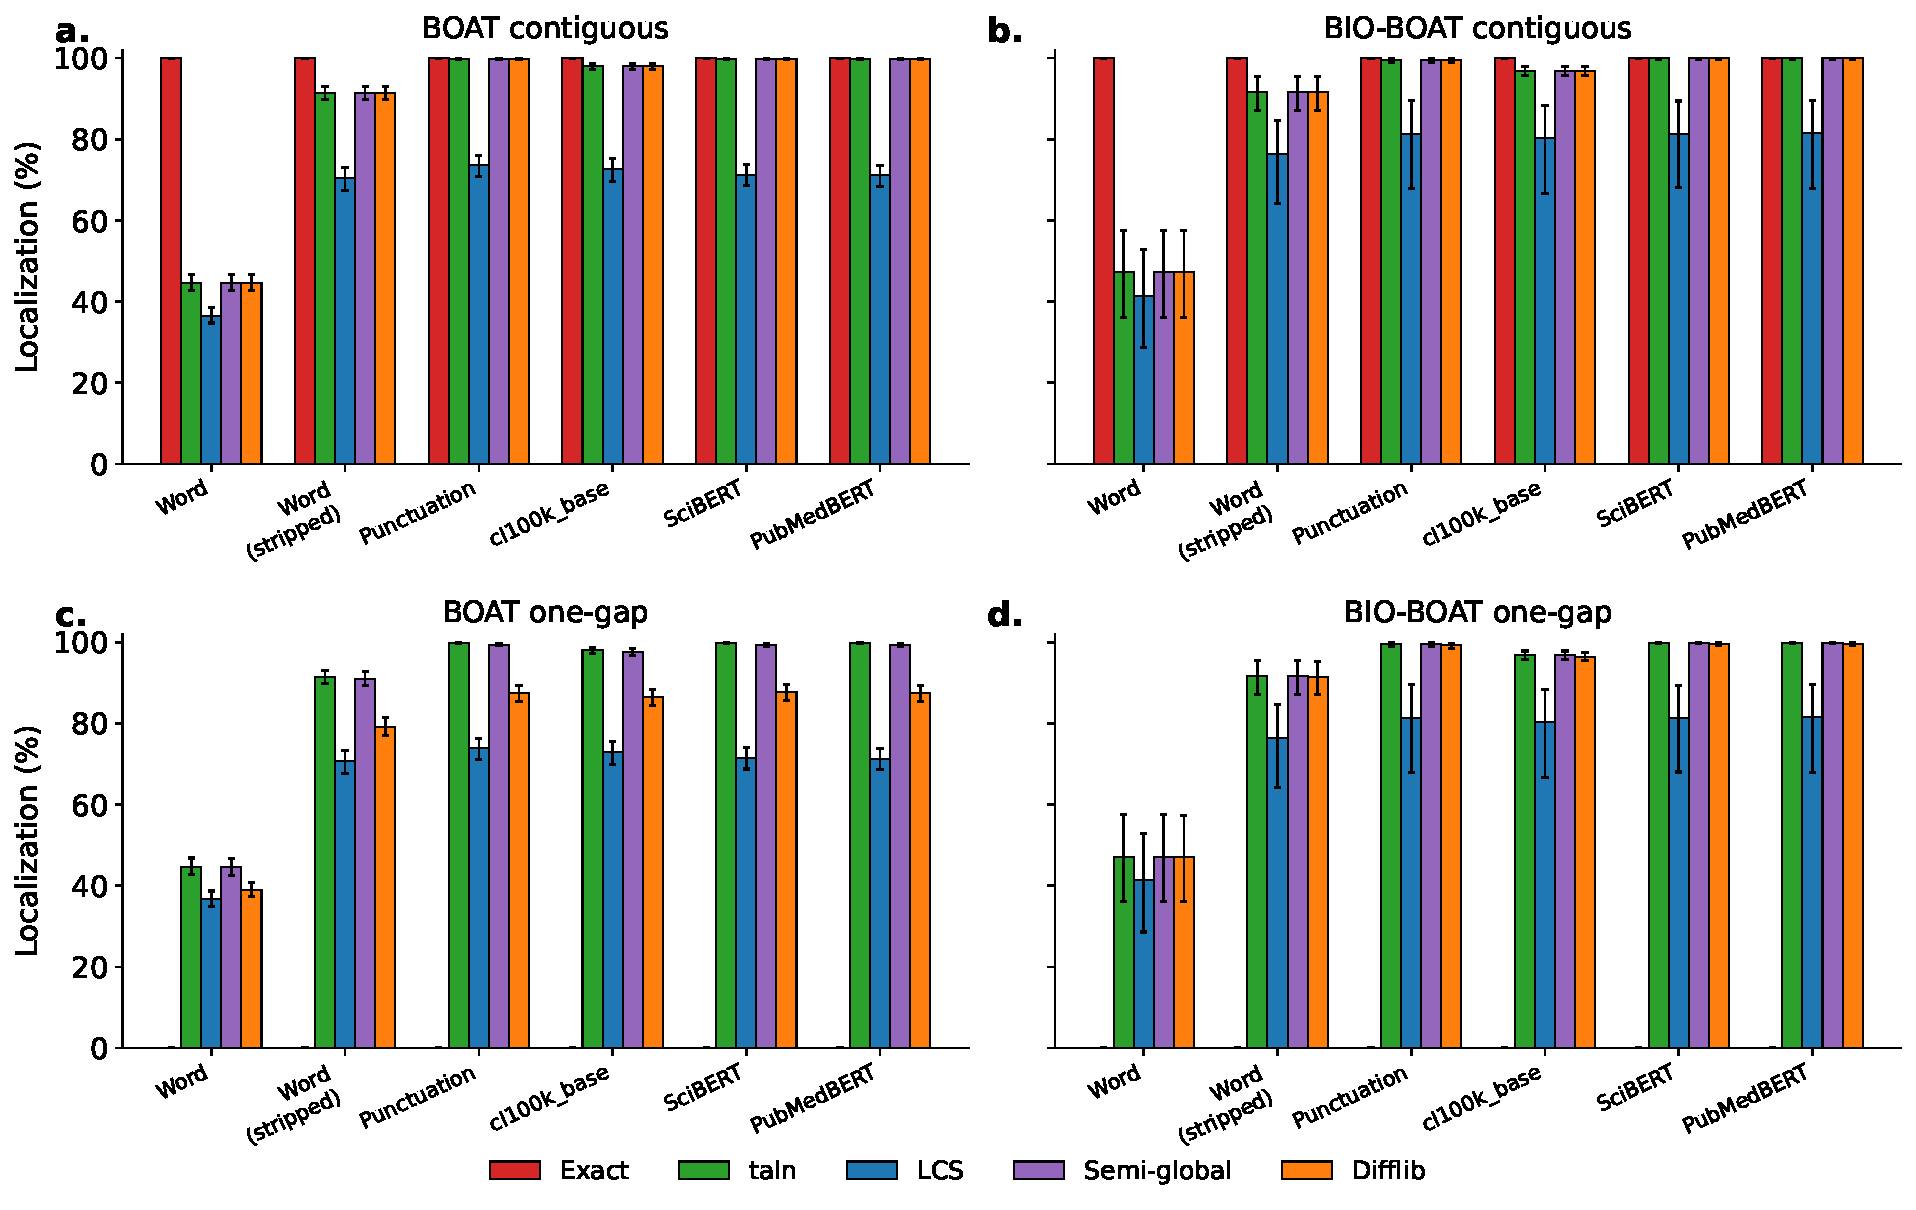
\includegraphics[width=\linewidth]{../../shared/figures/localization_accuracy.pdf}
    \caption{\textbf{Localization accuracy across methods and tokenizers.} Held-out localization for the same methods, tokenizers, and conditions as Supplementary Figure S1, with document-clustered 95\% confidence intervals. Localization requires a reconstructing alignment to start and end at a correct location in the original source.}
    \label{fig:s2}
\end{figure}

\end{document}
